\section{Physikalische Grundlagen}
\label{Kapitel:Rheologie}
In diesem Kapitel werden die grundlegenden Gleichungen vorgestellt, die in dieser Arbeit benutzt werden.
Dazu gehören sowohl Erhaltungssätze als auch rheologische Stoffgleichungen.

Rheologie ist die Wissenschaft über das Verhalten von Stoffen unter Einfluss äusserer Kräfte. Es wird untersucht wie Festkörper, Flüssigkeiten und Gase reagieren wenn sie deformiert werden.

Diese Arbeit beschäftigt sich mit der Simulation von Flüssigmörteln, weshalb hier nicht weiter auf Festkörper und Gase eingangen wird.
%
\subsection{Massen- und Impulserhaltung}
Die Massen- und Impulserhaltungsgleichung eines inkompressiblen Fluids kann in Matrix-Vektor Form als 
%
\newnot{symbol:boldu}
\newnot{symbol:rho}
\newnot{symbol:p}
\newnot{symbol:boldT}
%
\begin{equation}
    \label{eq:Massenerhaltung}
    \nabla \cdot \u = 0
\end{equation}
und
\begin{equation}
    \label{eq:Impulserhaltung}
    \rho \u _t + \rho \u \cdot \nabla\u = -\nabla p +\nabla \cdot \T + \rho \g
\end{equation}
%
geschrieben werden. Dabei ist $\u$ die Geschwindigkeit, $p$ der Druck, $\T$ der Spannungstensor, $\rho$ die Dichte und $\g$ eine auf das Fluid wirkende, volumetrische Kraft.
Der Einfachheit halber wird im Folgenden angenommen, dass $\g=0$.

Im allgemeinsten Fall kann der Spannungstensor eine beliebig komplexe Funktion des Orts und der Zeit $\T\left( \r,t \right)$ sein.
In dieser Arbeit wird diese Abhängigkeit eingegrenzt, indem $\T$ auf eine Funktion des Dehngeschwindigkeitstensors $\D$ und der Zeit beschränkt wird.
%
\newnot{symbol:boldD}
\newnot{symbol:t}
%
\begin{equation}
    \label{eq:Spannungstensor}
    \T = f\left( \D,t \right)
\end{equation}
%
Dabei ist 
\begin{equation}
    \label{eq:Dehngeschwindigkeitstensor}
    \D =\frac{1}{2} \left( \nabla \u + \nabla \u^T \right)
\end{equation}
%
\subsection{Konstitutive Gesetze}
Der Zusammenhang zwischen Viskosität und Dehngeschwindigkeitstensor sowie die viskoelastischen Eigenschaften werden durch konstitutive (stoffabhängige) Gesetze beschrieben.\\
Die Anforderungen an diese Gesetze sind vielfältig. Einerseits sollen sie die reellen Stoffeigenschaften möglichst gut beschreiben um realitätsnahe Modellierung zu ermöglichen. Andererseits sollen sie die zu lösenden Gleichungen nicht unnötig komplizieren und deshalb mit einfachen Zusammenhängen und wenig Parametern auskommen.\\
Aus diesen Anforderungen ist eine Vielzahl von Modellen entstanden, von denen einige nachfolgend aufgeführt werden. Weitere Modelle werden in \cite{boehme}, \cite{introtorheo} und \cite{comprheo} beschrieben.

\subsubsection{Zeitunabhängige Spannungen}
Ist $\T$ keine Funktion der Zeit, gilt $\T=f\left( \D \right)$.
Ein Spezialfall dieses Modelles ist die newtonsche Flüssigkeit, für die $\T=2\eta\D$, wobei hier auch oft von $\mu$ statt von $\eta$ gesprochen wird.

Statt $\T=f\left( \D \right)$ wird oft auch der Ausdruck
\begin{equation}
    \label{eq:TgeneralNewton}
    \T=\eta\left( \D \right)\cdot \D
\end{equation}
verwendet. Diese Darstellung ermöglicht es, von einem generalisiertem Newtonschen Fluid zu sprechen, bei dem die effektive Viskosität $\eta$ abhängig von den Dehngeschwindigkeiten $\left( \D \right)$ ist.

Wird angenommen, dass $\eta$ nur von der Summe aller Dehngeschwindigkeiten abhängt (isotrope Viskosität), kann man $\D$ mit der Scherrate $\gammap$ ersetzen:
\newnot{symbol:gammap}
\begin{equation}
    \label{eq:Scherrate}
    \gammap := \sqrt{2 \cdot \D\dipr\D}
\end{equation}
wobei
\begin{equation}
    \label{eq:doubleInnerProduct}
    \A\dipr\B := \sum_{i,j}{a_{ij}b_{ij}}
\end{equation}
das doppelte innere Produkt ist.

Mit Hilfe von \eqref{eq:Scherrate} lassen sich Modelle für die Funktion $F$ in zwei Kategorien unterteilen. Dilatante Fluide werden zähflüssiger wenn sie geschert werden, strukturviskose Fluide haben eine sinkende Viskosität für steigende Scherraten. 
Die Grenze zwischen diesen zwei Fällen ist das Newtonsche Fluid bei dem die Viskosität unabhängig von der Scherrate ist. 
Ein Spezialfall des strukturviskosen Fluids ist die Viskoplastizität, bei der erst nach dem Überschreiten einer Fliessgrenze $\tau_0$ ein Fliessvorgang möglich ist.\\
In Abbildung~\ref{fig:fliessKurven} sind diese Fliesskurven genannten Zusammenhänge dargestellt.
%
\begin{figure}
    \centering
    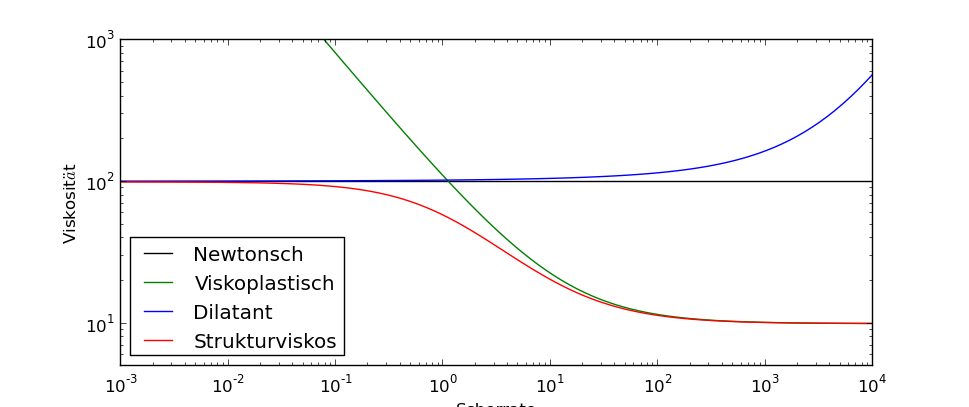
\includegraphics[width=\textwidth]{figures/Fliesskurven.png}
    \caption{Fliesskurven von verschiedenen Fluiden, dargestellt im doppelt logarithmischen Plot}
    \label{fig:fliessKurven}
\end{figure}
%
\begin{table}
    \centering
    \begin{tabular}{l l l}
        Modell & Fliessfunktion & Parameter \\
        \hline
        Newton & $\mu= \mbox{const}$ & $\mu$ \\ 
        Ostwald-de Waele & $\eta=K \gammap^{n-1}$ & $K,n$ \\ 
        Bingham-Modell & $\eta= \frac{\tau_0}{\gammap}+K $ & $\tau_0,K$ \\ 
        Carreau-Yasuda & $\eta=\eta_\infty+\left( \eta_0-\eta_\infty \right)\left[ \left( \gammap \right)^\alpha \right] ^{\frac{n-1}{\alpha}} $ & $\eta_0,\eta_\infty,\alpha,n$ \\ 
        Herschel-Bulkley & $\eta= \frac{\tau_0}{\gammap}+K\gammap^{n-1} $ & $\tau_0,K,n$
    \end{tabular}
    \caption{Fliessgesetze für zeitunabhängige Spannungen}
    \label{tab:Fliessgesetze}
\end{table}
%

Die scherratenabhängige Viskosität der von Hilti verwendeten Mörteln wurde schon in früheren Arbeiten untersucht. Diese zeigen ein viskoplastisches Verhalten, das sich am besten mit dem modifizierten Herschel-Bulkley Modell abbilden lässt:
\newnot{symbol:tau0}
\newnot{symbol:K}
\newnot{symbol:n}
\begin{equation}
    \label{eq:modHB}
    \eta\left( \gammap \right) = \tau_0 \frac{1-\exp \left( -m\gammap \right)}{\gammap}+K\gammap^{n-1}
\end{equation}
Die materialabhängigen Parameter sind dabei die Fliessgrenze $\tau_0$, die Konsistenz $K$ und der Fliessindex $n$. Der Parameter $m$ bestimmt das Verhalten des Modells bei sehr kleinen Scherraten und wurde in dieser Arbeit auf 1000 gesetzt.%Im Bild [\ref{fig:modHBKurven}] \todo{Bild} ist der Zusammenhang zwischen Viskosität und Scherrate für verschiedene Parametersets aufgetragen.

In Tabelle \ref{tab:Fliessgesetze} sind weitere dieser Fliessgesetze genannten Modelle aufgeführt.
%
\subsubsection{Zeitabhängige Spannungen}
Für viele Flüssigkeiten spielt nicht nur der aktuelle Zustand des Fluids eine Rolle, sondern auch die Geschichte der früheren Deformationen. Die konstitutive Gleichung $F$ ist also nicht mehr nur von $\D$ abhängig, sondern auch von der Zeit $t$ und der Verzerrungsgeschichte:
\begin{equation}
    \label{eq:Tviskoelastisch}
    \T\left( \D,t \right) = \underset{s\leq t}{F}\left[ \D(s) \right]
\end{equation}

Ein Modell um das Verhalten solch eines Stoffes zu beschreiben, ist das Maxwell-Modell.
Dabei wird das Material als eine Mischung aus einer viskosen Flüssigkeit und einer elastischen Feder beschrieben, deren Eigenschaften in Reihe geschalten sind. Eine schematische Darstellung ist in Abbildung~\ref{fig:Maxwell-Material} zu sehen.\\
Wird nun auf dieses Material eine Kraft in Form einer Spannung ausgeübt, nehmen beide Komponenten einen Teil davon auf, wobei die elastische Komponente diese als elastische Energie speichert und zu einem späteren Zeitpunkt wieder zurückgeben kann.
%
\begin{figure}
    \centering
    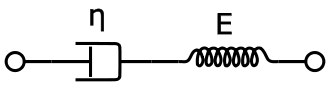
\includegraphics[width=0.5\textwidth]{figures/Maxwell-material.png}
    \caption{Schematische Darstellung des Maxwell - Materials}
    \label{fig:Maxwell-Material}
\end{figure}

Die resultierende Differentialgleichung für die Schubspannung $\T$ nimmt folgende Form an:
%
\newnot{symbol:lambda}
\begin{equation}
    \label{eq:maxwellModell}
    \T + \lambda \frac{\partial\T}{\partial t}=2\eta \D
\end{equation}
Die Voraussetzung dafür ist dass das Stoffverhalten als linear angenommen wird, indem nur Verzerrungen mit hinreichend kleiner Amplitude betrachtet werden. Zusätzlich muss noch die Annahme eines exponentiell schwindenden Gedächtnisses getroffen werden, das heisst der Einfluss von Verzerrungen auf die aktuelle Spannung nimmt mit der Zeit exponentiell ab.
Wie schnell dieser Einfluss abnimmt, hängt dabei von der Relaxationszeit $\lambda$ ab.

Eine Erweiterung dieses Modells ist das Oldroyd-B Modell, bei dem statt die partielle die kontravariante Ableitung $\overset{\nabla}{\T}$ verwendet wird:
\begin{equation}
    \label{eq:oldroydModell}
    \T + \lambda \overset{\nabla}{\T}=2\eta \D
\end{equation}
wobei
\begin{equation}
    \label{eq:upperconvectedDerivative}
    \overset{\nabla}{\T} = \frac{D}{Dt}\T-\left[ \nabla u^T\cdot \T \right]-\left[ \T\cdot \nabla u \right] 
\end{equation}
Diese Modifikation dient dazu, Drehungen und Verzerrungen des Fluides in der Differentialgleichung zu berücksichtigen.

Das in dieser Arbeit verwendete Modell für viskoelastische Fluide muss zusätzlich zu der Zeitabhängigkeit auch die stark scherratenabhängigen Effekte berücksichtigen können.\\
Dazu in der Lage ist das White-Metzner Modell. Dieses ist eine Erweiterung des Oldroyd-B Modelles, bei dem zusätzlich $\lambda$ und $\eta$ eine Funktion von $\gammap$ sind:
\begin{equation}
    \label{eq:whiteMetznerModell}
    \T + \lambda\left( \gammap \right) \overset{\nabla}{\T}=2\eta\left( \gammap \right) \D
\end{equation}
Dabei können im Allgemeinen für die Funktionen $\lambda$ und $\eta$ die selben Modelle wie für die nicht zeitabhängigen Gesetze verwendet werden.
In dieser Arbeit wurde für $\eta$ das schon bewährte modifizierte Herschel Bulkley Modell \eqref{eq:modHB} implementiert.\\
Für die Relaxationszeit $\lambda$ wird auf Empfehlung des Rheologiespezialisten von Hilti das Carreau-Yasuda Modell verwendet:
%
\begin{equation}
    \label{eq:carreauYasuda}
    \lambda \left( \gammap \right) = \eta_{\inf} +\left( \eta_0 - \eta_{\inf} \right) \left( 1+\left( L\gammap \right)^\alpha \right)^{\frac{n_{\lambda}-1}{\alpha}}
\end{equation}
%
Die Parameter $\eta_{\inf}$, $\eta_0$, $L$, $\alpha$ und $n_{\lambda}$ sind dabei wieder materialabhängig. 
%
%\subsubsection{Strukturviskosität}
%%
%\subsubsection{Viskoelastizität}
%%
%\subsubsection{Konstitutive Gesetze}
